\chapter{Mitigation methods}
This chapter introduces our mitigation strategies for lowering the overall latency.
We decided to focus on decreasing the LimeSDR loopback delay and the GNU radio processing delays as it is evident from our results that they are the major contributors to the overall latency.
The chapter first investigates the reasons for the LimeSDR loopback delay, followed by discussion of our method of decreasing the LimeSDR FPGA packet size.
We then discuss our strategy for modifying the GNU radio scheduler parameter for specifying the maximum number of data elements processed in one execution of each block.
The design of the experiment for evaluation of our strategies is discussed in the last section.

\section{LimeSDR loopback delay}
We found the LimeSDR loopback delay is quite significant in our results from Experiment 2.
Although the software delays are also high, the difference in results across the two host computer provides us with enough reason to argue that these delays are because of the limitations of the host computer hardware configuration.
These can be mitigated to some extent by buying higher processing resources.
The LimeSDR loopback delay is constant across both the host computers and hence can be classified as a property of the LimeSDR-USB platform.
We decided to focus on the LimeSDR loopback delay as it is a fundamental delay of the platform and will affect the performance of any system designed using the LimeSDR-USB platform.\\

In order to have a closer understanding, we segment the LimeSDR loopback delay into LimeSDR platform delays and bus transfer delay.
\ac{USB} 3.0 provides data bandwidth of 4 Gbps and if the entire bandwidth is available for the data transfer, it would take $\frac{4096*8}{4 Gbps} = 8.192 \mu s$ for a single LimeSDR FPGA packet of 4096 bytes.
This is much smaller than the overall LimeSDR loopback delay, hence this delay can be safely ignored.
Hence, we can approximate the LimeSDR loopback delay as the LimeSDR platform delay, which can be decomposed into processing delays and buffering delays in the LimeSDR-USB platform.
The processing delays can be neglected as the main processing tasks of the hardware logic is to convert streams of samples to sample data packets and vice versa.
This conversion involves buffering of sample data and is dependent on the implementation of the data paths in the LimeSDR FPGA.
Hence, it is necessary to have a closer understanding of the FPGA implementation of these data paths.\\

The RX data path is responsible for converting sample streams to packets, it incurs buffering delays as it has to wait for the samples which are regulated by the sampling rate used.
On the other hand, the TX data path receives data packets from the host computer using a high speed parallel interface.
So all the data necessary for creating the sample stream is available to the TX data path and it doesn't experience buffering delays.
With this in mind, we focus more on the RX data path.


\subsection{Analytical understanding of the LimeSDR FPGA RX data path}
In this subsection, the report concentrates on highlighting the implementation details of the RX data path in the LimeSDR FPGA and describing an mathematical equation for the RX data path delays to find out the suitable choice of parameters for decreasing the RX data path delay.

\begin{figure}[h!]
\centering
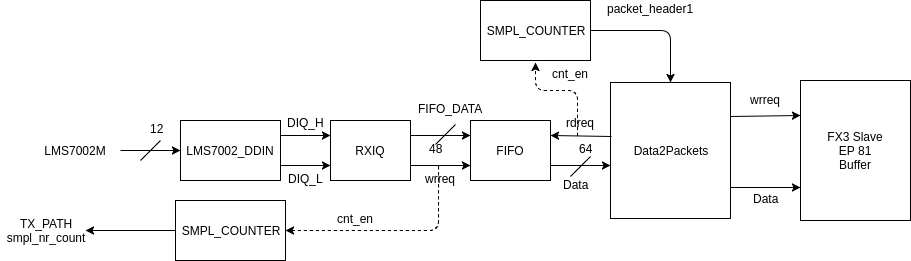
\includegraphics[width=\textwidth]{Figure/DATA2PACKETS.png}
\caption{LimeSDR FPGA RX Path}
\label{RX_Path}
\end{figure}

\subsubsection{RX Path:}

Figure \ref{RX_Path} shows the overview of the RX Path implementation on the LimeSDR-USB \ac{FPGA}.
The hardware logic is described as a number of processing blocks connected via signals to make the design modular and understandable.
This paragraph uses quoted text and italics to represent processing blocks and signals respectively.\\

Sample data from the LMS7002M is captured by the "LMS7002\_DDIN", which uses an ALT DDIO IP (ref alt ddio ip) block to capture in-phase and quadrature samples at double data rate.
% This means that incoming data stream is latched both at the positive and negative edges of the clock.
"LMS7002\_DDIN" latches the sample data collected at the postive and negative edge of the clock into two different components: \textit{DIQ\_H} and \textit{DIQ\_L} repectively.
It introduces one clock delay between the LMS7002M Sample Stream, and the \textit{DIQ\_L}, \textit{DIQ\_H} outputs.\\

The "RXIQ" block is responsible for arranging the individual components into a single data structure of In-phase component of a sample followed by its Quadrature component.
It consumes four component data coming from the "LMS7002\_DDIN" block and arranges them in a sequence: \textit{DIQ\_L},\textit{DIQ\_H}, \textit{DIQ\_L}, \textit{DIQ\_H}.
"RXIQ" takes one clock cycle for latching these component data coming from the "LMS7002\_DDIN".
It takes three clock cycles for producing the structure.
Finally, the output is latched after one clock cycle from the internal output register.
It writes this structure every two clock cycles to the "FIFO" by enabling the \textit{wrreq} signal.\\
% This means effectively one IQ sample is then sent to the "FIFO" every clock cycle. \\

The first "SMPL\_COUNTER" is a 64-bit counter which increases its count every time "RXIQ" asserts the \textit{wrreq} for writing new data samples to the "FIFO". 
The count is sent to the TX Path to track the number of produced samples. 
The second "SMPL\_COUNTER" is also a 64 bit counter which is enabled when the data is read from the "FIFO" by the "DATA2PACKETS" block.
It increases its count every clock cycle when the \textit{rdreq} signal is '1'.\\

The "FIFO" uses the FPGA RX \ac{PLL} output as the read and write clocks.
The RX PLL frequency is equal to the sampling rate of the data converters.
The read enable is controlled by the "RXIQ" using the \textit{wrreq} signal, so two new samples are written in two clock cycles of the RX PLL.
On the write side, the "DATA2PACKETS" controls the write enable signal (\textit{rdreq}).
The "FIFO" receives the 48-bit data samples, stores them in a \ac{FIFO} structure and keeps track of how many samples have been loaded into the \ac{FIFO}.
The "FIFO" takes one clock cycle for latching the input.
The counter for the number of elements loaded into the FIFO is updated five clock cycles after the data has been latched.
\\

The "DATA2PACKETS" block is responsible for converting data samples into packets.
It mainly consists of two \ac{FSM}.
The first  \ac{FSM} controls the read and write signal for the input and output blocks.
It monitors the amount of data in the "FIFO", and when it is greater than the amount of data in one packet it asserts the \textit{rdreq} signal.
It takes two clock cycles for the "DATA2PACKETS" to register that the number of data elements in the "FIFO" is sufficient for one \ac{FPGA} packet.
The first \ac{FSM} takes two more clock cycles to generate the \textit{rdreq} signal after that.\\ 

The second \ac{FSM} arranges the data in the FPGA data packet structure.
It latches the value of the sample count from the second "SMPL\_COUNTER" when the first \ac{FSM} asserts the \textit{rdreq} signal.
It adds the sample count and different flags as meta-data for each LimeSDR \ac{FPGA} packet. 
Once, the first \ac{FSM} determines there is enough space to write the data in the FX3 buffer, it enables the \textit{wrreq} signal and writes 64 bits of data every clock cycle.
The second \ac{FSM} takes 6 clock cycles to output the first data element read from the "FIFO" after the \textit{rdreq} has been generated by the first \ac{FSM}.\\

\subsubsection{RX Path Delays}
The delays introduced by the individual blocks has been highlighted in the previous paragraph and visualized using Figure \ref{timing_diagram}
All these delays have been measured by simulation of the RX data path in Modelsim.

\begin{figure}[h!]
\centering
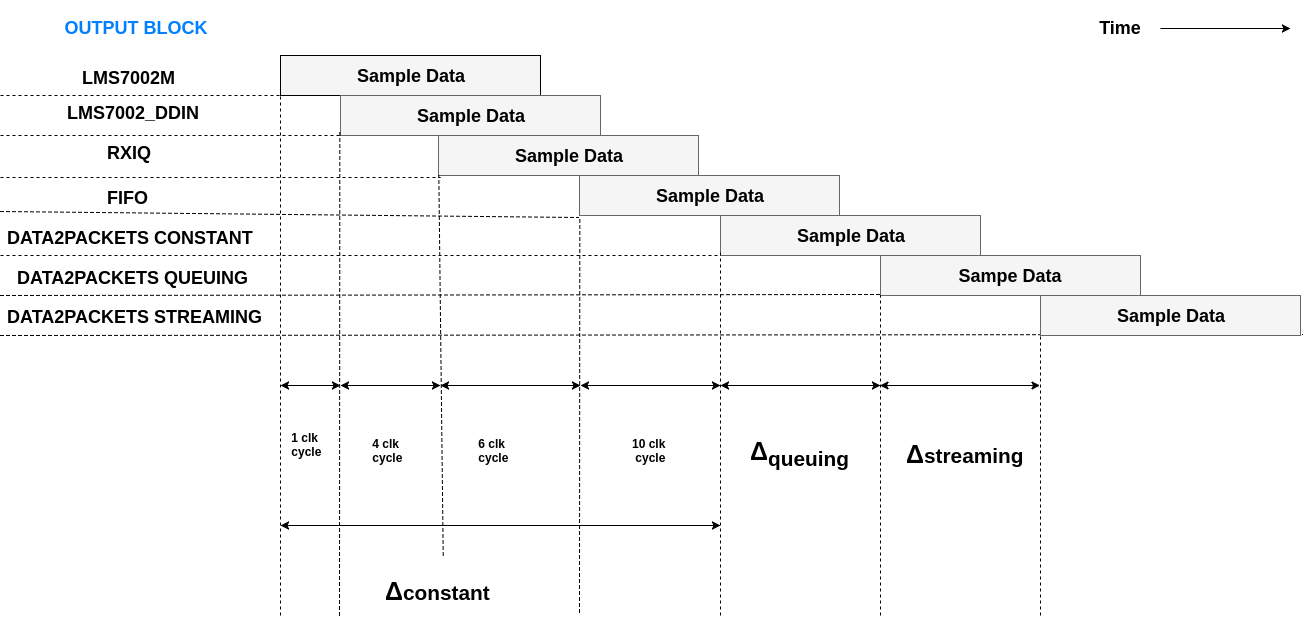
\includegraphics[width=\textwidth]{Thesis/Figure/Timing_Diagram.png}
\caption{LimeSDR RX data path timing diagram}
\label{timing_diagram}
\end{figure}

\begin{itemize}
\item{Delay introduced by the "LMS7002\_DDDIN" block : 1 clock cycle}
\item{Delay introduced by the "RXIQ" block: 5 clock cycles ; 1 clock cycle each for input and output latching, and 3 clock cycles for forming the data structure.}
\item{Delay introduced by the "FIFO" block: 6 clock cycles ; 1 clock cycle for input latching; 5 clock cycles for the increment of internal counter}
\item{Delay introduced the the "DATA2PACKETS" block: 10 clock cycles ; 4 clock cycles for generation of \textit{rdreq} signal and 6 clock cycles for output of the first data element read from the "FIFO"}
\end{itemize}

The report will refer to these block delays as constant delays.
We define sample index as the number of samples that has entered the RX data path, with the first sample from the LMS7002M entering the RX data path having sample index of zero. 
The constant delay is 22 clock cycles for even index samples, and 21 clock cycles for odd index samples.
The even index samples take one more clock cycle more as it has to wait for the the odd index samples in the "RXIQ" block.
The constant delays can be represented as:\\

\begin{subequations} \label{eq1}
\begin{align}
	sampl_{rel} = sampl_{abs} \ \text{mod} \ N \label{eq1.1}\\ 
  packet\_number= \floor*{\frac{sampl_{abs}}{N}} \label{eq1.2}\\
  \Delta_{constant} = \frac{22 - \floor*{sampl_{rel} \ \text{mod} \ 2 }}{f_s} \label{eq1.3}
\end{align}
  
\end{subequations}

N = Number of samples in one packet, $f_s$ is the \ac{FPGA} RX PLL frequency, $sampl_{rel}$ is the relative sample index, $sampl_{abs}$ is the absolute sample index in Equation \ref{eq1}, \texttt{mod} is modulus operator and $\floor*{.}$ is the floor operator.

For example, with N=1020, $sampl_{abs}$ = 8000, packet\_number would be $\floor*{\frac{8000}{1020}} = 7$, and $sampl_{rel}$ would be  $8000 \ mod \ 1020 = 860$. \\
 
In addition to the constant delays, there are two more delays that needs to be considered.
They are the Queuing Delay and the Streaming Delay.
The data elements in the "FIFO" has to wait until there is sufficient data for a single packet.
This waiting time is being referred to as Queuing Delay.
The Queuing Delay is dependent on the relative samle index.
If the element is the $N^{th}$ sample, it has to wait for N clock cycles, where N is the number of samples in one packet.
If the element is the $N-1^{th}$ sample, it needs to wait only for one more sample, that is two clock cycles.

\begin{equation} \label{eq2}
\Delta_{queuing} = \frac{N - 2 \times \floor*{\frac{sampl_{rel}}{2}}}{f_s}
\end{equation}
 
The "DATA2PACKETS" block outputs two samples in one clock cycle, streaming out the stored FIFO data sequentially.
The time a sample has to wait to be streamed is being referred as the streaming delay.
The streaming delay is also dependent on the arrival time of the sample which is equivalent to the absolute sample index.
If the sample has relative sample index $N$, it is the first data element of a packet, it doesn't need to wait for any sample to be streamed ahead of it, so it has zero streaming delay.
On the other hand, the sample with relative sample index $N-1$ needs to wait for N-3 samples to streamed first, before it is outputted together with the $N-2^{th}$ sample.

\begin{equation}\label{eq3}
\Delta_{streaming} =\frac{\floor*{\frac{sampl_{rel}}{2}}}{f_s}
\end{equation} 


The total delay can be calculated as :\\
\begin{subequations}\label{eq4}
\begin{align}
\Delta_{total}= \Delta_{constant} + \Delta_{queuing} + \Delta_{streaming} \\
\Delta_{total}= \frac{22 +  N - \floor*{\frac{sampl_{rel}}{2}} - \floor*{sampl_{rel} \ \text{mod} \ 2}}{f_s}
\end{align}
\end{subequations}

\subsection{Decreasing $\Delta_{total}$} \label{decrease}

In order to decrease $\Delta_{total}$ as described by equation \ref{eq4}, we can either decrease $N$ or increase $f_s$ as $sampl_{rel}$ is dependent on the arrival time of the sample, which we cannot control.
Since the primary focus of the project was to evaluate the performance of IEEE 802.15.4 networks, we keep $f_s$ as 4 MHz.
Another workaround might be increasing $f_s$ and using software decimation, but this leads to higher software processing delays as the software now needs to process higher number of data samples.
$\Delta_{total}$ can also be decreased by decreasing N which will increase the amount of data transferred through the USB interface as every LimeSDR FPGA packet is packed with 16 bytes of packet header.
This increase in the size of USB transfer data can easily be tolerated by the USB interface as in the default case we are using roughly 4\% of the total bandwidth provided by the USB interface.
Because of this, we concentrate on decreasing N.\\

We do a min-max analysis of $\Delta_{total}$ using equation \ref{eq4} to observe the impact of $N$ on the overall latency and jitter.
The incoming data sample depending on its sample index can experience any delay between the minimum and maximum values of \ref{eq4} with equal probability.
Because of this, the maximum amount of jitter contributed by the FPGA RX path can be estimated by finding the difference between the minimum and maximum values of equation \ref{eq4}.
Table \ref{min-max} shows the approximate results using  equation \ref{eq4} for four different values of $N$: 1020, 764, 508 and 252.
These values of $N$ were chosen as they correspond to samples needed for 4kB, 3kB, 2kB and 1kB of USB Transfer size respectively with 16 bytes of LimeSDR FPGA packet header.\\
\begin{table}[h]
\centering
\begin{tabular}{ c c c c }
N &  Min & Max & Max-Min\\
\hline
1020 & 133  & 260.5 & 127.5 \\
764 & 101  & 196.5 & 95.5 \\
508 & 69 & 132.5 & 63.5 \\
252 & 37 & 68.5 & 31.5 \\
\end{tabular}
\caption{Min-Max analysis for different values of N}
    \label{min-max}
\end{table}

% \subsection{Implementation}

In order to experimentally validate the results from Table \ref{min-max}, we configure the TX and RX datapaths of the LimeSDR \ac{FPGA} to use 1 kB, 2 kB, 3 kB and 4 kBas the LimeSDR FPGA packet size.
The Cypress EZ-FX3 initializes the DMA channel between the GPIF II socket and USB socket with \ac{DMA} buffer size of 4 kB.
The USB Transfer of lower LimeSDR FPGA packet sizes has to wait until one DMA buffer size is filled as the USB socket is notified only when a DMA buffer is full.
Because of this, in principle we are still using the default LimeSDR FPGA packet size of 4kB.
We modified the DMA buffer descriptor on the EZ-FX3 microprocessor to make one DMA buffer size same as the LimeSDR FPGA packet size.
As the minimum configurable DMA buffer size of the Cypress EZ-FX3 is 1kB, we set the LimeSDR FPGA packet sizes as multiples of the 1kB.
Finally, the LimeSDR driver on the host computer is modified to handle the reduced size of the LimeSDR FPGA packet structure.

\section{Software Chain Delays}

Although the software chain delays is heavily dependent on the host computer processing resources, how the execution of GNU Radio blocks is controlled by the scheduler also has an impact on the software chain delays.
In case of software implementation of signal processing algorithms, the number of data elements to be processed has a direct correlation to the time taken by the algorithm, with higher number of data elements resulting in higher processing time.
In GNU Radio, as most of the blocks are signal processing blocks the number of data elements processed in one execution of these blocks impacts the latency through the flow-graph.
If one of the GNU radio blocks in a flowgraph takes significantly longer processing time, then the buffers of the downstream blocks run dry.
In this case, the scheduler fails to pipeline the block executions properly thereby increasing its latency.
Decreasing the processing time for the GNU Radio block might lead to better pipelining lowering the latency of the flowgraph.
Each execution of the a GNU Radio block is associated with a number of control signals as described in Section 2.1.3.
Increasing the number of executions of a GNU Radio block will lead to increase of the number of control signals, which will increase the processing overhead.
We need to investigate the impact of the number of elements processed by the flowgraph to find the trade off between lower latency and increased processing overhead.\\


GNU Radio scheduler allows us to control the maximum number of data elements processed in one execution of a GNU Radio processing block by using \texttt{max\_noutput\_items} method.
This method caps the maximum number of data elements but the scheduler can still decide on the actual number of elements processed in one execution.
We decided to set the \texttt{max\_noutput\_items} for one the entire TX and RX flowgraphs, instead of tuning this parameter for each block.
This will help the GNU radio scheduler to optimize the flowgraphs for latency in case there is any processing block having longer processing delays.


\section{Experiment 4: Evaluation of Mitagation Methods} \label{exp4}
The final experiment is designed to evaluate the impact of smaller LimeSDR FPGA packet size and maximum number of elements processed by a GNU Radio block on the latency and component delays.

\begin{itemize}
    \item \textbf{Objective} This experiment is designed to evaluate our mitigation methods described previously using the experimental setup described in Figure \ref{component_setup}.
    This experiment will help in analyzing which configuration among the measured configuration of USB Transfer size and GNU Radio execution size provides the best results.
    Since this experiment is done across both the host computers, the impact of processing resources will also be studied with respect to our mitigation strategies.
    \item \textbf{Input Parameters} The experiment uses two input parameters:
    \begin{itemize}
        \item \textbf{LimeSDR FPGA Packet Size} Following the discussion in \ref{decrease}, we set the LimeSDR packet size to 1kB, 2kB, 3kB and 4kB (default case).
        \item \textbf{GNU Radio \texttt{n\_output\_items}} We set the GNU Radio flowgraph's \texttt{n\_output\_items} to 1000, 2000 and  4000 data elements. 
    \end{itemize}
    \item \textbf{Output Metric} Latency and Component Delays as described in Experiment 2.
    As the best configuration of the input parameters for the host computers will be dependent on its processing resources, the percentage of CPU and memory usuage will also be measured using \texttt{pidstat}.
    \item \textbf{Design of Experiment} The experiment collects 999 latency and component delays over 500 seconds. The time period of the message source is set to 500 ms, the message source generates 10 bytes data payload. \texttt{Pidstat} collects percentage of CPU and memory usage every one second (least possible). The sampling rate is set to 4 MHz as we are evaluating the latency with respect to IEEE 802.15.4 networks.
\end{itemize}

\section{Throughput Analysis}
Both of our mitigation strategies revolve around the idea of decreasing the transfer time or processing time.
This decrease comes at the cost of increase in the number of times data has to be transferred and number of times a block needs to be executed which results in increased processing overhead.
Since we are dealing with multi-core processors, we assume that the increase in processing overhead can be compensated with the better pipelined processing providing us better latency.
In this case, although we might achieve lower latency, the throughput of the entire system can be affected because of the increase of the processing overhead for handling the same amount of data.
We need to evaluate the how our mitigation strategies effect the throughput of the system.\\

We send a controlled data payload size from the periodic message source using experimental setup shown in Figure \ref{Experimental_Setup_Flow_Digram}.
The time when the SFD is detected is noted as $T_{SFD}$, when the complete packet is decoded, we note the time-stamp as $T_{Complete}$.
As we control the data payload size, we know the size of data decoded between the two timestamps.
We can then define throughtput as;
\begin{equation} \label{eq:throughput}
    Throughput= \frac{data\_payload\_size}{T_{Complete} - T_{SFD}}
\end{equation}
This throughput definition provides the MAC layer throughput as we are calculating our throughput using the MAC data payload size.\\

The best combination of input parameters as determined from the results of Experiment 4 for the desktop computer is taken as the input parameter for this measurement.
We compare the throughput for this configuration to that of the default configuration of the LimeSDR platform.
We set the data payload size to the 112 bytes with the time period of the message source is set to 500ms. The experiment was ran for 500 seconds resulting in 999 throughput measurements.





